\chapter{State of the Art}\label{cap:conceptual}

This chapter presents the state of the art relevant to the development of a multimodal
system for sexism detection under the Learning with Disagreement paradigm. The analysis
is organized into five complementary sections: Section 2.1 examines the evolution of
sexism and hate speech detection, from early text-only methods to current multimodal
approaches; Section 2.2 analyzes multimodal learning architectures applied to memes
and short-form video, together with their limitations; Section 2.3 introduces the Learning
with Disagreement paradigm and soft-label training as an alternative to majority-vote
labeling; Section 2.4 reviews annotator modeling and reliability estimation techniques,
from early competence-estimation models to recent demographic-aware approaches; and
Section 2.5 synthesizes these four perspectives, identifying the gaps that this dissertation
aims to address.

\section{Sexism and Hate Speech Detection}\label{sec:sexism-hate-speech-detection}

Sexism and hate speech detection has evolved over the past
decade, following the broader progression of natural language processing and computer
vision techniques. Understanding this evolution is essential for situating system proposed in this dissertation.

Early approaches to sexism and hate speech detection relied entirely on textual content.
\cite{waseem2016hateful} framed hate speech detection as a supervised classification
problem over surface-level linguistic features, such as character n-grams and word
embeddings, applied to short social media posts. These text-only methods proved effective
for explicit forms of hate speech, characterized by unambiguous slurs or overtly aggressive
language, but struggled to capture more implicit or context-dependent expressions, where
meaning depends on cultural references, sarcasm, or visual elements absent from the text
itself.

The introduction of multimodal benchmarks revealed the limitations of unimodal
approaches for social media content in which discriminatory meaning arises specifically
from the interaction between text and image.~\cite{kiela2020hateful} demonstrated, through
the Hateful Memes Challenge, that meme classification systems relying solely on text or
solely on image features consistently underperform relative to systems that jointly reason
over both modalities, since a meme's message frequently depends on the juxtaposition of
an image with an unrelated or contradictory caption. This finding established multimodal
reasoning as a necessary, rather than optional, component of hateful and sexist content
detection in visual social media formats.

More recently, the object of detection has extended beyond static images to short-form
video, a format that introduces additional temporal and auditory dimensions.~\cite{arcos2024tiktok}
proposed one of the first multimodal frameworks specifically targeting sexism detection
in TikTok videos, combining textual transcripts, audio features, and visual frames, and
showed that this combination substantially outperforms text-only baselines on video
content, where tone of voice, background music, and visual context frequently carry
sexist meaning that is entirely absent from the spoken or written text. Complementing this
direction,~\cite{degrazia2025mused} introduced a Spanish-language video dataset annotated
with modality-specific labels, explicitly measuring the contribution of each modality to
human sexism judgments. Their results show that visual cues play a decisive role in the
recognition of implicit or indirect sexism, cases in which annotators relying on the text
transcript alone frequently disagree with annotators who have access to the full video, underscoring
both the necessity of multimodal analysis and the inherently subjective nature
of the task.

Taken together, this body of work traces a clear trajectory from unimodal, explicit hate
speech detection towards multimodal, context-dependent sexism characterization across
increasingly rich media formats. This trajectory motivates a closer examination of the
multimodal learning architectures that make such joint reasoning possible, which is the
focus of the next section.

\section{Multimodal Learning for Memes and Video}\label{sec:multimodal-learning-memes-video}

Building on the need for cross-modal reasoning established in the previous section, this
section examines the architectures developed to jointly process textual, visual, and, for
video content, auditory information, along with the specific limitations that motivate the
architectural choices adopted in this dissertation.

Contrastive vision-language pre-training has become a foundational technique for
representing images and text within a shared embedding space.~\cite{radford2021learning}
introduced CLIP, a model trained on large-scale image-text pairs using a contrastive
objective, producing visual and textual encoders whose representations are directly comparable through cosine similarity. While CLIP was designed as a general-purpose vision-
language model rather than one tailored to hateful or sexist content, its representations
have become a common starting point for multimodal meme classification, given the
strong alignment they provide between image and text semantics without requiring paired
supervision specific to the target task.

Building on this foundation,~\cite{kumar2022hateclipper} proposed Hate-CLIPper, which
explicitly models cross-modal interactions between CLIP-derived image and text features
through a feature interaction matrix, rather than treating them as independent inputs to be
concatenated. This architecture specializes the general-purpose alignment learned by CLIP
into a task-specific representation for hateful meme detection, and established a strong
baseline for subsequent multimodal meme classification systems. More recent submissions
to sexism detection shared tasks have explored an alternative direction, leveraging large
pretrained multimodal models directly through fine-tuning or prompting rather than designing specialized fusion mechanisms~\cite{aiwizards2026}. Both directions, however, share
a common limitation for the sexism detection setting: neither explicitly models the annotation disagreement that characterizes sexism as a subjective task, treating each meme as
having a single correct label to be predicted.

Extending multimodal reasoning to short-form video introduces additional architectural
challenges, since video content combines temporal, visual, textual, and auditory signals that must be aligned and fused.~\cite{tong2022videomae} proposed VideoMAE,
a self-supervised video encoder trained via masked autoencoding, which learns effective
spatio-temporal representations from a comparatively small number of labeled videos, making it particularly suitable for tasks such as sexism detection where large annotated video
corpora are not available. For the auditory component,~\cite{radford2023whisper} introduced Whisper, a speech recognition and audio representation model trained on large-scale
weakly supervised data, robust to the noisy, non-studio audio conditions typical of user-
generated video content. Combining video, audio, and text encoders into a single system
requires a fusion strategy capable of handling the resulting high-dimensional, heterogeneous representation space, as well as robustness to cases where one modality is degraded
or entirely missing, a common occurrence in real-world video content where audio may
be silent, absent, or uninformative.

A recurring design decision across this literature concerns how modality-specific representations should be combined. Approaches based on cross-modal attention allow each
modality to dynamically weigh evidence from the others, offering, in principle, a more
expressive fusion mechanism. In practice, however, such mechanisms require substantial
training data to learn meaningful attention patterns, and can collapse to near-uniform
weighting when trained on comparatively small, specialized datasets such as those used for
sexism detection. Simpler fusion strategies, such as concatenating pooled representations
from each modality before a shared classification head, have been shown in several settings
to match or exceed the performance of more elaborate attention-based mechanisms under
these data constraints, while being considerably lighter to train and less prone to overfitting.

This trade-off between architectural expressiveness and data efficiency directly informs
the fusion strategies adopted for both the meme and video systems developed in this
dissertation, detailed in Chapters 4 and 5, respectively. The next section turns to a distinct
but complementary challenge: how these multimodal systems should be trained when the
labels themselves reflect genuine disagreement among annotators.

\section{Learning with Disagreement and Soft-Label Training}\label{sec:learning-disagreement-soft-label}

The previous sections established that sexism detection requires multimodal reasoning
and that annotators frequently disagree on whether content is sexist. This section explains
how this disagreement can be explicitly incorporated into model training, rather than
discarded through majority vote.

The conventional approach to supervised classification collapses multiple annotator
judgments into a single label, typically via majority vote, treating any remaining
disagreement as noise to be resolved rather than as signal to be modeled.
\cite{davani2022dealing} show that this practice discards systematic information: for
genuinely subjective tasks, disagreement often correlates with identifiable factors such
as the content's ambiguity or the annotators' own backgrounds, rather than reflecting
random labeling error. Collapsing this variation into a single label therefore produces
models that are confidently wrong on precisely the instances where human judges
themselves were uncertain or divided.

The Learning with Disagreement (LeWiDi) paradigm addresses this limitation by
reframing the prediction target itself. Instead of predicting a single aggregated label, a
model trained under this paradigm predicts the full distribution of annotator judgments
for each instance, commonly referred to as a soft label. \cite{uma2021learning} survey
this shift across NLP and computer vision tasks, arguing that treating disagreement as
signal, rather than noise, is particularly important for inherently subjective tasks such as
sexism, hate speech, and irony detection, where no single ground truth may exist independently
of the annotator's perspective.

\begin{figure}[htb]
    \centering
    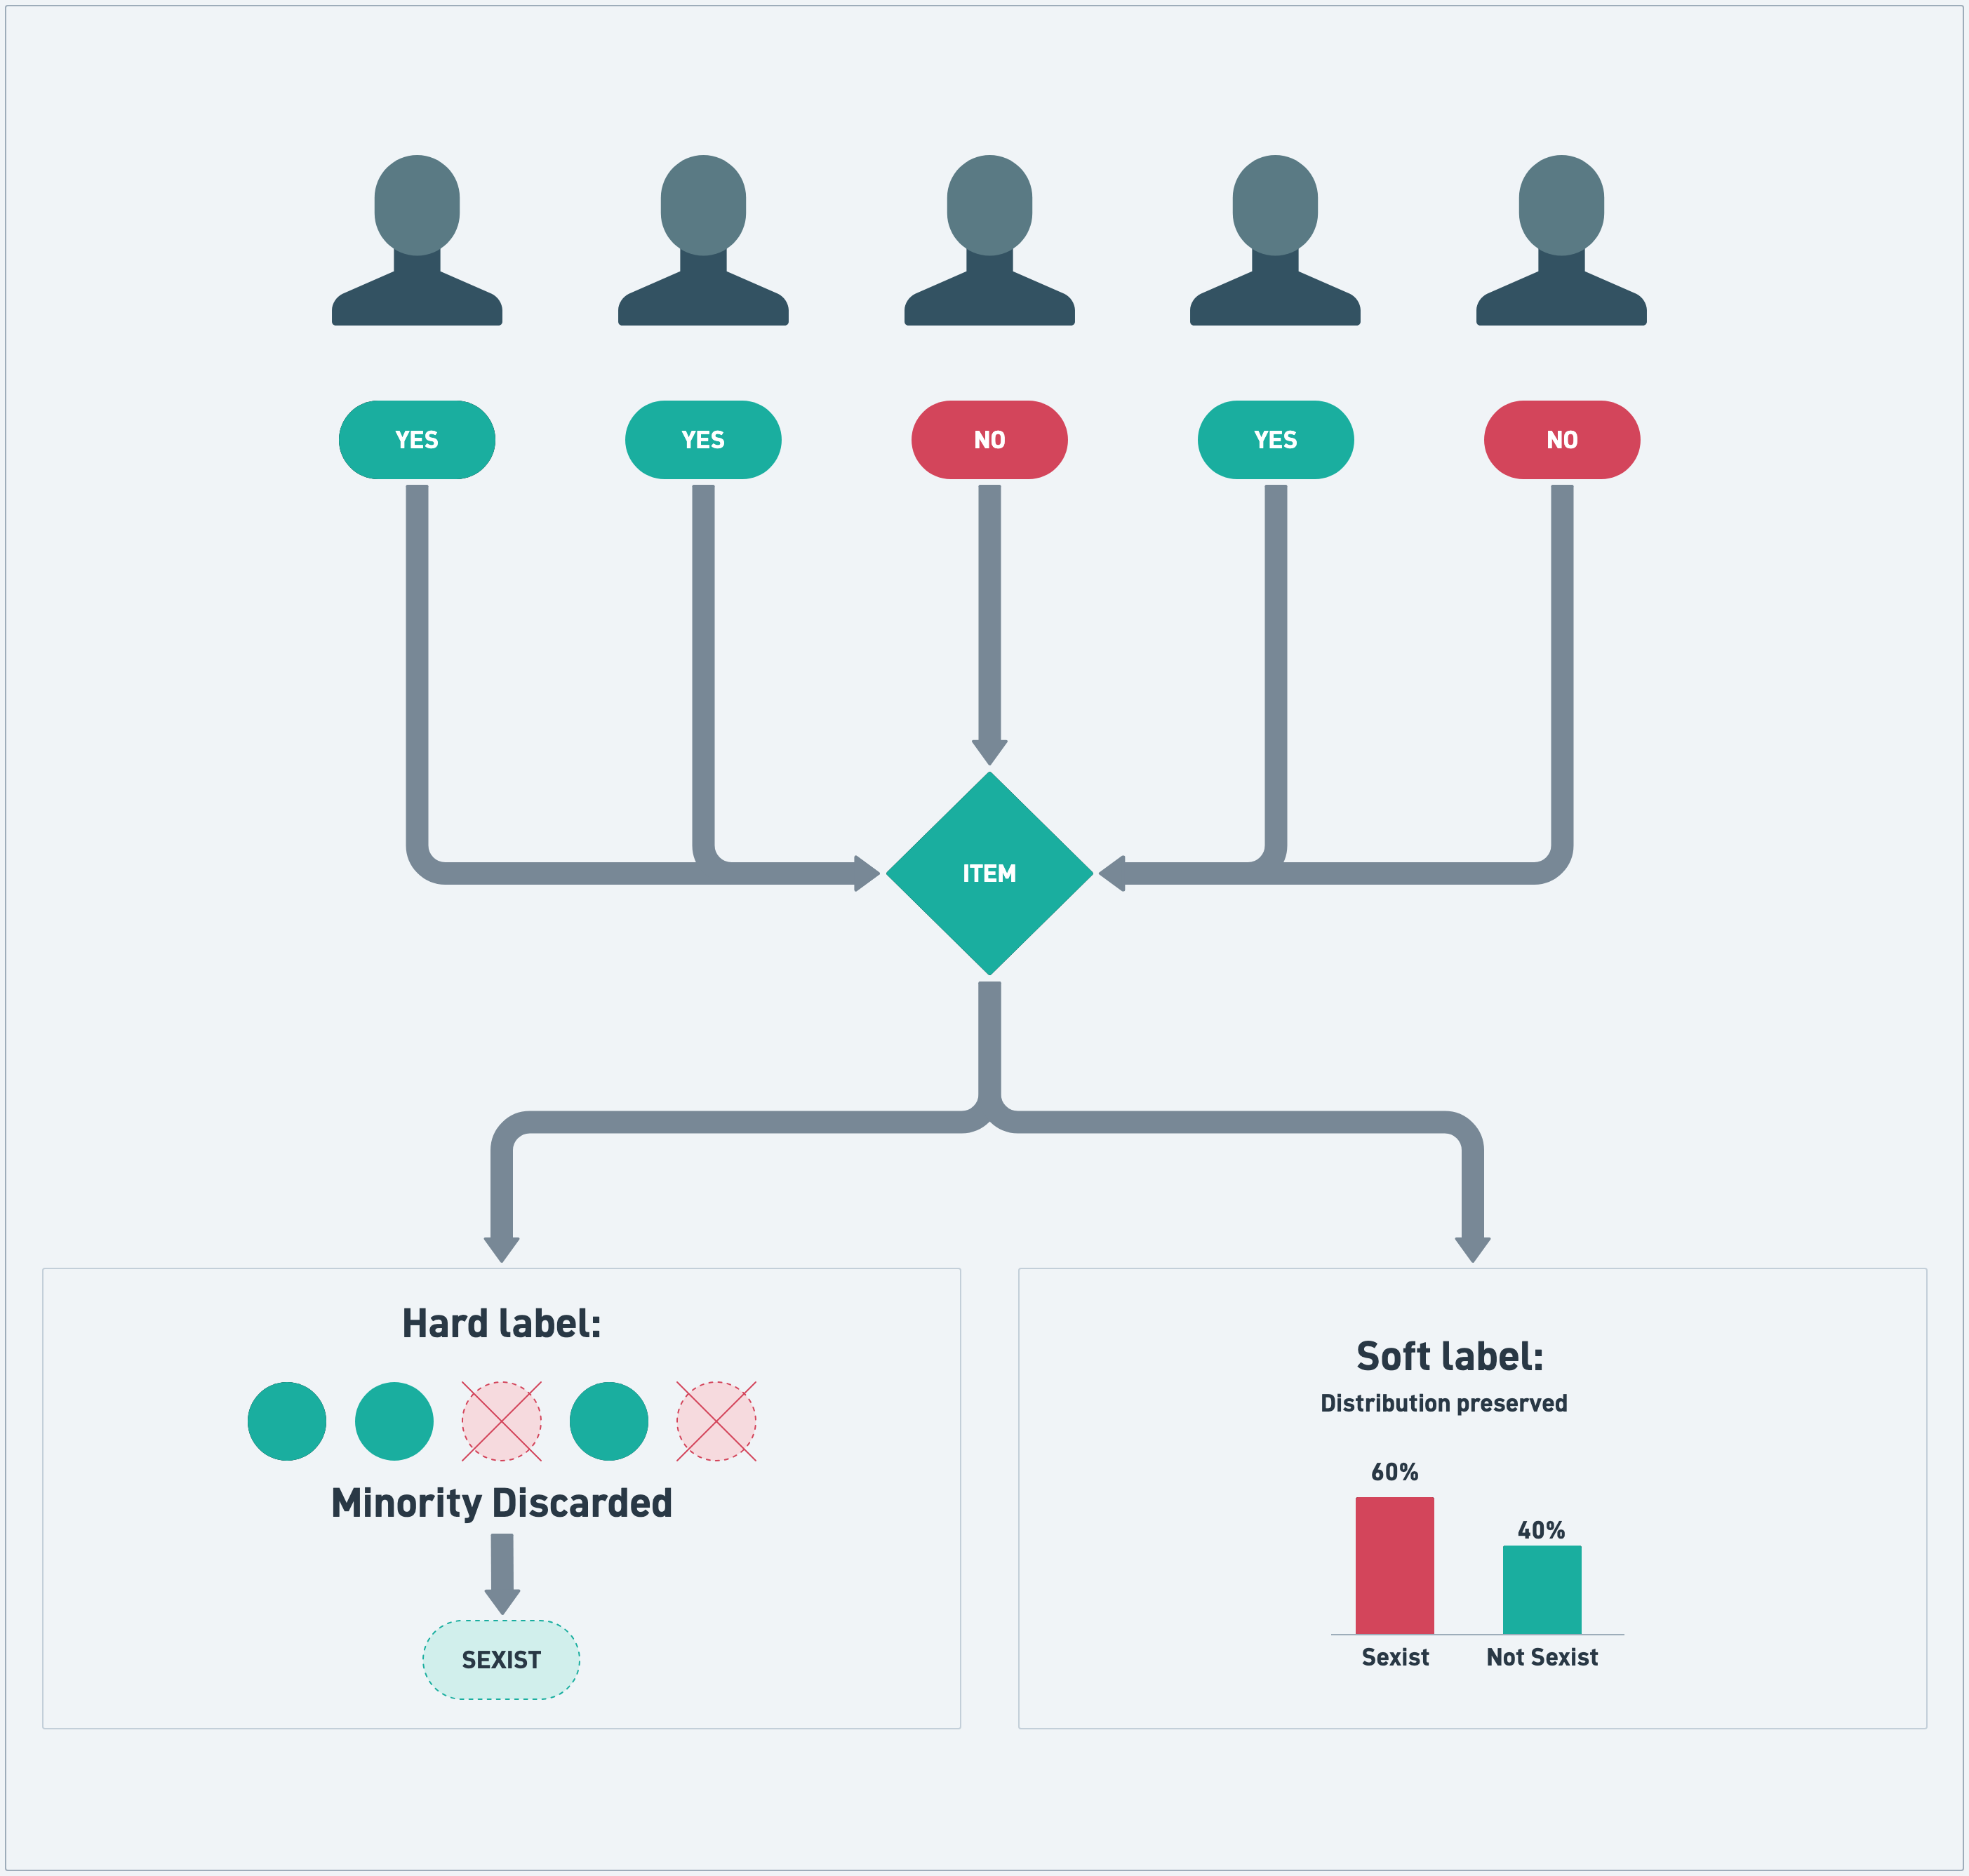
\includegraphics[width=0.65\textwidth]{images/soft_labels.png}
    \caption{Conceptual comparison between hard-label and soft-label training. Five
    annotators cast individual judgments on the same content; the hard-label approach
    collapses this into a single majority-vote label and discards the minority votes,
    while the soft-label approach preserves the full distribution of annotator judgments.}
    \label{fig:hard-soft-label}
\end{figure}


\cite{plank2022problem} further formalizes this
position, characterizing human label variation as a property of the data-generating process
itself, rather than as a symptom of poor annotation quality, and arguing that evaluation
protocols should be adapted according to that.

The LeWiDi shared task series has served as the primary place for developing and
benchmarking soft-label training methods. \cite{leonardelli2023lewidi} organized the second
edition of this task around subjective NLP classification problems, training and evaluating
systems directly against soft-label distributions rather than hard labels, and reporting that
directly optimizing for the target distribution, typically via a distributional loss such as
cross-entropy or Manhattan distance between predicted and observed label distributions,
consistently outperforms training on aggregated labels and subsequently calibrating the
output. The third edition of this task, \cite{leonardelli2025lewidi}, further distinguishes
between two complementary evaluation paradigms: predicting the population-level distribution
of judgments for an instance, and predicting the specific interpretation of an
individual annotator, a distinction that is directly relevant to the annotator reliability
modeling developed in this dissertation.

Physiological signals collected alongside subjective annotations represent a further
extension of this paradigm, offering a potential behavioral correlate of the perceptual
and affective processes underlying disagreement itself, an avenue that remains largely
unexplored in the sexism detection literature \cite{exist2026overview}.

Training directly on soft labels, rather than majority-vote labels, is the approach adopted
throughout the meme and video systems developed in this dissertation, detailed in
Chapters 4 and 5. However, soft-label training alone does not distinguish between two
fundamentally different sources of the disagreement it preserves: genuine ambiguity in the
content, and inconsistency or unreliability on the part of individual annotators. This
distinction is the focus of the next section.



\section{Annotator Modeling and Reliability Estimation}\label{sec:annotator-modeling-reliability-estimation}

The previous section established that training directly on soft labels preserves annotator
disagreement as informative signal. However, not all of this disagreement reflects genuine
ambiguity in the content: some of it results from annotator inconsistency, carelessness, or
error. This section reviews the evolution of techniques for estimating annotator reliability,
from early statistical models to recent demographic-aware approaches, motivating the
annotator reliability studies developed in this dissertation.

The foundational approach to modeling annotator reliability was proposed by
\cite{dawid1979maximum}, who introduced an Expectation-Maximization algorithm for
jointly estimating the true label of each item and the error rate of each annotator from
multiple noisy annotations, without requiring access to ground truth during training. This
formulation established the basic premise that underlies most subsequent work in this area:
annotators are not equally reliable, and this reliability can be estimated directly from
patterns of agreement and disagreement within the annotation data itself.

\cite{hovy2013mace} extended this idea with MACE, a model that explicitly distinguishes
between annotators who are honest but occasionally noisy and annotators who behave
as spammers, assigning a competence score to each annotator based on how consistently
their labels align with the inferred consensus. \cite{paun2018comparing} later provide a
systematic comparison of Bayesian models of annotation, including Dawid-Skene and
MACE-style formulations, showing that the choice of model has a measurable impact
on the quality of the inferred ground truth, particularly under sparse or unbalanced
annotation patterns, a condition common in large-scale crowdsourced datasets.

These early reliability models, while effective at identifying unreliable annotators,
were not designed to distinguish reliability from genuine, systematic disagreement rooted
in annotator perspective. \cite{davani2022dealing} argue that collapsing annotator
identity into a single competence score can obscure meaningful patterns of disagreement
that correlate with annotator background, and propose multi-task architectures that
predict each annotator's individual judgment rather than a single aggregated reliability
estimate. This shift towards perspective-aware modeling motivated subsequent work
that incorporates annotator identity or demographic information directly into the
learned representation. \cite{gordon2022jury} introduce jury learning, which models
every annotator individually and composes configurable juries with a specified demographic
composition, allowing practitioners to control which perspectives are reflected in the
final prediction. \cite{xu2025demmoe} propose DEM-MoE, which routes predictions
through expert subnetworks conditioned on annotator demographics, explicitly capturing
group-level and intersectional variation in a more structured form than individual
annotator embeddings.

A common limitation across these embedding-based approaches is that they learn
representations tied to the specific annotators seen during training, and therefore
cannot generalize to annotators who did not contribute to the training set.
\cite{ignatev2025hypernetworks} address this parametric efficiency and generalization
bottleneck by replacing fixed annotator embeddings with hypernetwork-generated
adapters, allowing the model to adapt to new annotators without retraining from
scratch. This limitation is particularly relevant for annotator reliability modeling: a
system that only recognizes annotators present during training cannot estimate the
reliability of new annotators contributing to a dataset after deployment, restricting its
practical applicability. \cite{ivey2025nutmeg} propose NUTMEG, a more recent approach
that separates genuine signal from noise in annotator disagreement while explicitly
preserving systematic, perspective-driven disagreement rather than treating all variation
as a symptom of unreliability, addressing a key shortcoming of earlier competence-based
models. \cite{vandermeer2024annotator} take a complementary, active-learning perspective,
proposing annotator-centric selection strategies that account for individual annotator
characteristics when deciding which items and which annotators to prioritize for further
labeling in subjective NLP tasks.

Taken together, this progression reveals a trajectory from purely statistical competence
estimation, through individual annotator embeddings, towards demographic-conditioned
approaches capable of generalizing beyond the specific annotators observed during
training. This last property, generalization to unseen annotators via demographic
conditioning, rather than fixed annotator identity, is the central design principle
adopted by the annotator reliability layer developed in this dissertation, detailed in
Chapter 6.

\section{Towards Demographic-Aware, Disagreement-Preserving Systems}\label{sec:demographic-aware-disagreement-preserving}

This section synthesizes the four perspectives reviewed in this chapter, allowing us to
identify the specific gaps that this dissertation addresses. The analysis is structured around
two complementary axes: first, the extent to which a system integrates multiple modalities
rather than relying on text alone; second, the extent to which a system preserves annotator
disagreement as prediction target rather than collapsing it into a majority-vote label.

Multimodal learning has substantially advanced the detection of hateful and sexist content
in memes and, more recently, in short-form video, as reviewed in Sections 2.1 and 2.2.
Architectures built on contrastive vision-language encoders and specialized cross-modal
fusion mechanisms consistently outperform unimodal baselines when discriminatory
meaning arises from the interaction between modalities \cite{kiela2020hateful,
kumar2022hateclipper}. However, these systems are almost universally trained on
majority-vote labels, treating sexism as a task with a single correct answer per instance,
despite the inherently subjective nature of the judgment being modeled.

Conversely, the Learning with Disagreement paradigm, reviewed in Section 2.3, has
demonstrated that training directly on soft-label distributions produces better-calibrated
predictions on genuinely ambiguous content \cite{uma2021learning, leonardelli2023lewidi}.
However, this line of work has developed almost entirely within unimodal, text-based NLP
tasks, and its extension to multimodal settings, where disagreement may arise jointly from
visual, textual, and auditory ambiguity, remains comparatively unexplored.

A third, largely independent line of work, reviewed in Section 2.4, has focused on
modeling annotator reliability and demographic background directly, moving from
early competence-estimation models towards demographic-conditioned architectures
capable of generalizing to annotators unseen during training \cite{xu2025demmoe,
ignatev2025hypernetworks}. This work has, so far, been developed independently of both
the multimodal fusion techniques discussed in Section 2.2 and the soft-label training
objectives discussed in Section 2.3, rather than as an integrated component of a single
system.

\begin{figure}[htb]
    \centering
    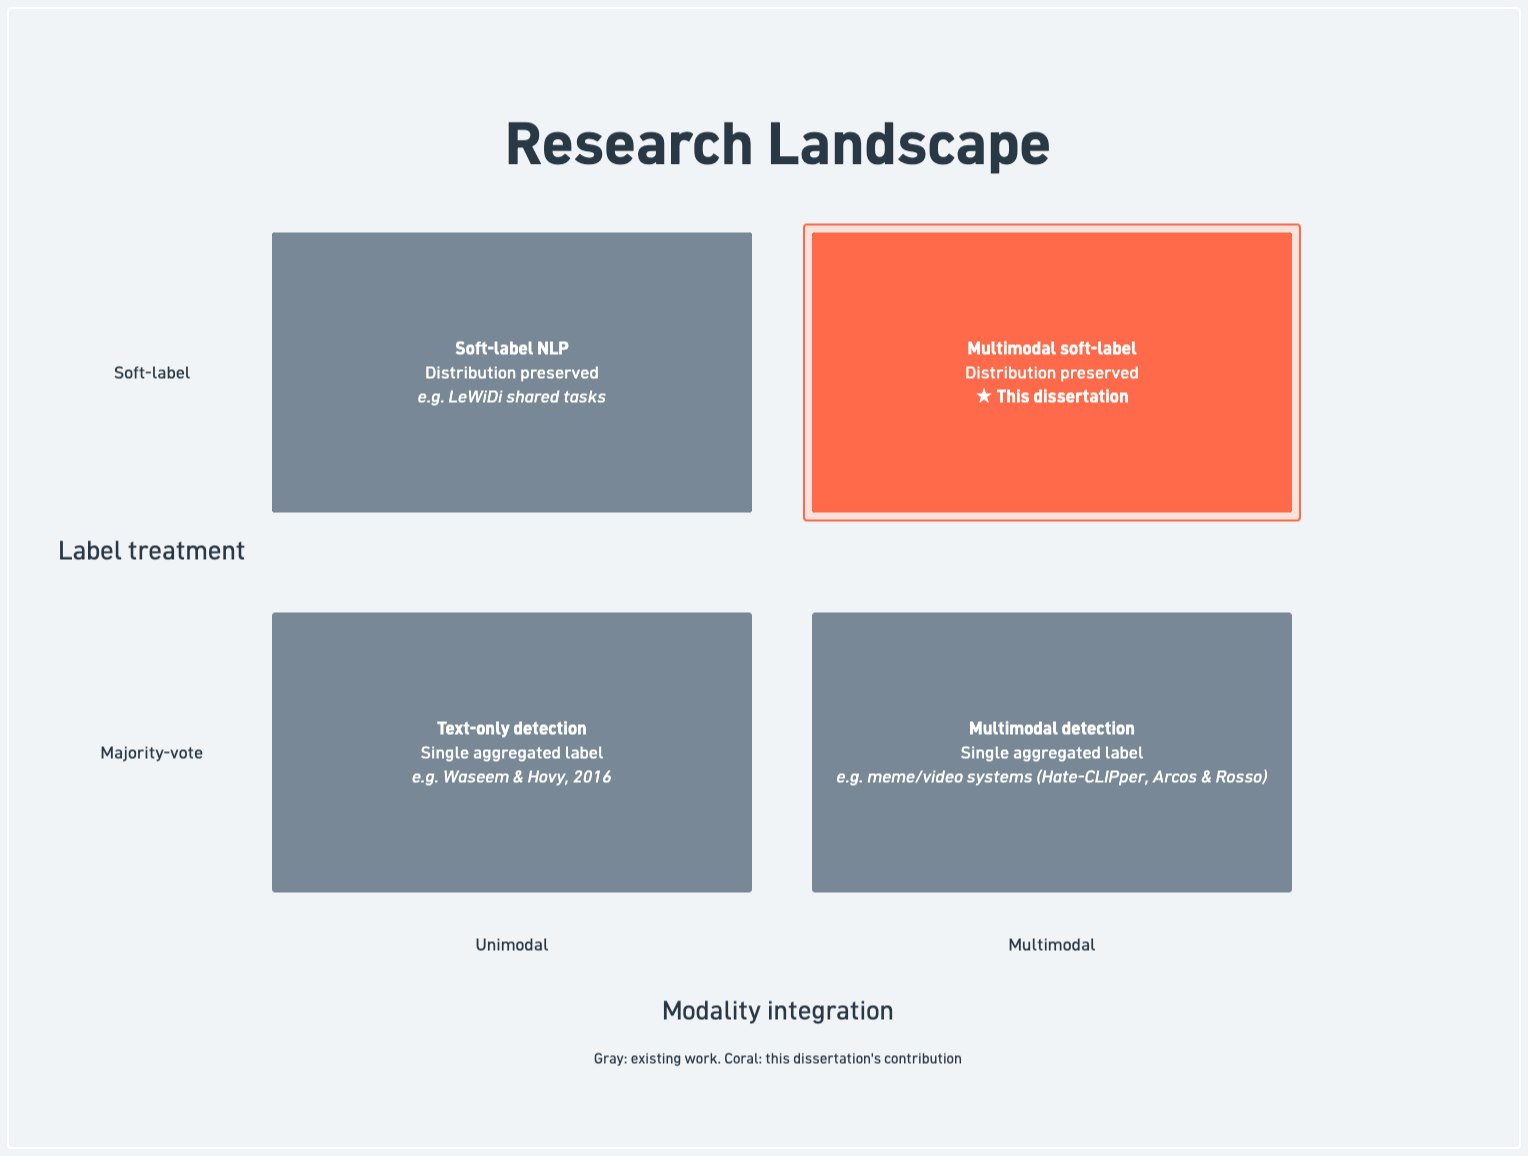
\includegraphics[width=0.85\textwidth]{images/landscape.png}
    \caption{Research landscape for sexism detection approaches.}
    \label{fig:landscape}
\end{figure}

The intersection of these three lines of work, illustrated in Figure~\ref{fig:landscape},
remains largely unexplored. Existing multimodal systems for sexism and hate speech
detection predominantly occupy the majority-vote quadrant of this landscape, regardless
of how many modalities they integrate. Systems trained under the Learning with
Disagreement paradigm predominantly remain unimodal. Demographic-aware annotator
reliability models, in turn, have not yet been integrated into multimodal, soft-label-trained
architectures for sexism detection specifically, nor extended to short-form video content
enriched with physiological signals \cite{exist2026overview}.

This dissertation proposes to address this gap by developing a multimodal system for
sexism detection in memes and short-form video that is trained directly on soft-label
distributions and incorporates a demographic-conditioned annotator reliability layer
capable of generalizing to unseen annotators. The system leverages the cross-modal
fusion strategies identified in Section 2.2 as most effective under limited training data,
while adopting the soft-label training objective established in Section 2.3, and extends
the demographic-aware reliability modeling reviewed in Section 2.4 into a jointly trained,
multimodal setting. Chapters 4 and 5 detail the resulting architecture for memes and
video, respectively, and Chapter 6 details the annotator reliability layer that completes
this integration.